\documentclass[14pt]{article}
\usepackage[utf8]{inputenc}
\usepackage[T2A]{fontenc}
\usepackage[uzbek]{babel}
\usepackage{amsmath, amssymb}
\usepackage{geometry}
\usepackage{graphicx}
\usepackage{xcolor}
\usepackage{hyperref}
\usepackage{tasks}
\usepackage{tcolorbox}
\tcbuselibrary{skins, breakable, theorems}
\usepackage{fancyhdr}
\usepackage{lastpage}
\usepackage{enumitem}
\usepackage{paracol}
\usepackage{ifthen}
\usepackage{needspace}

% Tanjens va kotanjens uchun buyruqlar (ruscha uslub saqlangan)
\newcommand{\tg}{\operatorname{tg}}
\newcommand{\ctg}{\operatorname{ctg}}

% Geometriya sozlamalari
\geometry{a4paper, left=10mm, right=10mm, top=20mm, bottom=20mm, headheight=15pt}

% Ranglar palitrasi
\definecolor{primary}{RGB}{52, 152, 219}
\definecolor{secondary}{RGB}{46, 204, 113}
\definecolor{accent}{RGB}{155, 89, 182}
\definecolor{lightbg}{RGB}{248, 249, 250}
\definecolor{taskborder}{RGB}{230, 230, 230}
\definecolor{optionbg}{RGB}{240, 242, 245}

% Sahifa asosiy foni
\pagecolor{lightbg}

% Giperssilka sozlamalari
\hypersetup{
    colorlinks=true,
    linkcolor=primary,
    urlcolor=primary,
}

% Kolontitullar
\pagestyle{fancy}
\fancyhf{}
\fancyhead[L]{\textcolor{primary}{\textbf{MathCore | MOCK Test-10}}}
\fancyhead[R]{\textcolor{secondary}{Abdunazarov M.X.}}
\fancyfoot[L]{\href{https://t.me/Math_Core_Dtm_MS_Att}{\textcolor{primary}{MathCore}}}
\fancyfoot[R]{\href{https://t.me/Abd_mardon}{\textcolor{secondary}{@Abd\_mardon}}}
\fancyfoot[C]{\textcolor{gray}{\thepage/\pageref{LastPage}}}
\renewcommand{\headrulewidth}{0.5pt}
\renewcommand{\headrule}{\hbox to\headwidth{\color{primary}\leaders\hrule height \headrulewidth\hfill}}
\renewcommand{\footrulewidth}{0.5pt}
\renewcommand{\footrule}{\hbox to\headwidth{\color{secondary}\leaders\hrule height \footrulewidth\hfill}}

% Titul sahifasi
\title{\Huge \textbf{\textcolor{primary}{MOCK Test-10}}}
\author{\textcolor{secondary}{Abdunazarov M.X.}}
\date{}
\newenvironment{dd}{\begin{center}}{\end{center}}
% Savol kartochkasi uslubi
\newtcolorbox{questionbox}[2][]{
    enhanced,
    breakable,
    colback=white,
    colframe=primary,
    coltitle=white,
    fonttitle=\bfseries\large,
    title={Masala \hfill \textcolor{white}{#2}},
    attach boxed title to top left={xshift=5mm, yshift=-2mm},
    boxed title style={size=small, colback=primary, sharp corners},
    sharp corners,
    boxrule=0.5pt,
    left=5mm,
    right=5mm,
    top=5mm,
    bottom=5mm,
    drop fuzzy shadow,
    #1
}

% Javob variantlari uslubi
\newlist{options}{enumerate}{1}
\setlist[options]{
    label=\textbf{\Alph*)},
    leftmargin=*,
    itemsep=2pt,
    topsep=5pt,
    before={\vspace{2mm}\begin{tcolorbox}[
        colback=optionbg,
        colframe=white,
        sharp corners,
        boxrule=0pt,
        left=2mm,
        right=2mm,
        top=2mm,
        bottom=2mm,
    ]},
    after={\end{tcolorbox}\vspace{2mm}},
}

% Rasmlar uchun
\newcommand{\questionimage}[2][0.5\linewidth]{%
    \begin{center}
        \includegraphics[width=#1]{#2}
    \end{center}
}

% Savolni rasm bilan kiritish buyrug'i
\newcommand{\questionitem}[4]{%
    \needspace{5cm}
    \begin{questionbox}{#1}
        #2
        \ifx&#3&%
        \else
            \questionimage{#3}
        \fi
        \begin{options}
            #4
        \end{options}
    \end{questionbox}
}

\begin{document}

% Titul sahifasi
\maketitle
\begin{center}
    
\includegraphics[width=0.2\textwidth]{logo.png} \\[5mm]
    \textcolor{gray}{\small Telegram: \href{https://t.me/Math_Core_Dtm_MS_Att}{@Math\_Core\_Dtm\_MS\_Att}}
\end{center}
\vspace{5mm}
% Masala 1
\begin{questionbox}{1}
    Quyidagi tasdiqlar to'g'ri yoki noto'g'riligini aniqlang:
    \begin{enumerate}
        \item[(I)] Agar \(x_1, x_2, x_3\) — \(ax^3 + bx^2 + cx + d = 0\) tenglamasining ildizlari bo'lsa, u holda \(x_1 + x_2 + x_3 = -b/a\).
        \item[(II)] Markazi \(O(a; b)\) va radiusi \(R\) bo'lgan aylana tenglamasi: \((x + a)^2 + (y + b)^2 \le R^2\).
        \item[(III)] Murakkab funksiya hosilasi uchun: \((g(f(x)))' = f'(x) g(f'(x))\).
    \end{enumerate}
    \begin{options}
        \item I – to'g'ri, II – noto'g'ri, III – noto'g'ri
        \item I – noto'g'ri, II – noto'g'ri, III – to'g'ri
        \item I – to'g'ri, II – to'g'ri, III – noto'g'ri
        \item I – noto'g'ri, II – to'g'ri, III – noto'g'ri
    \end{options}
\end{questionbox}

% Masala 2
\begin{questionbox}{2}
    2001 dan kichik bo'lgan va raqamlari yig'indisi 2 ga teng bo'lgan nechta tub son bor?
    \begin{options}
        \item 5
        \item 4
        \item 2
        \item 3
    \end{options}
\end{questionbox}

% Masala 3
\begin{questionbox}{3}
    \(ABC\) uchburchakda \(\angle B = \angle D\) (rasm), \(|AC| = 12\), \(|EC| = 4\) va \(S_{CDE} = 12\). \(S_{ABED}\) ni toping.
\begin{dd}
        \centering
        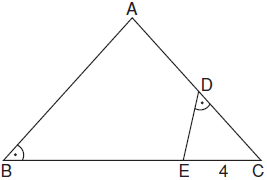
\includegraphics[width=0.5\linewidth]{eq.png}
    \end{dd}
        \begin{options}
        \item 108
        \item 48
        \item 98
        \item 96
    \end{options}
\end{questionbox}

% Masala 4
\begin{questionbox}{4}
    1 dan 1000 gacha bo'lgan natural sonlar ketma-ket yozilgan: 123...1000. Ushbu yozuvda 7 raqami necha marta qatnashgan?
    \begin{options}
        \item 200
        \item 270
        \item 280
        \item 300
    \end{options}
\end{questionbox}

% Masala 5
\begin{questionbox}{5}
    \(7^3 + 11 \cdot 7\) ni 6 ga bo'lgandagi qoldiqni toping.
    \begin{options}
        \item 3
        \item 0
        \item 2
        \item 1
    \end{options}
\end{questionbox}

% Masala 6
\begin{questionbox}{6}
    Natural \(a\) uchun \(a^2 - 1 = 8^7 (2^{19} + 1)\) bo'lsa, \(\frac{a-1}{64^3}\) ni toping.
    \begin{options}
        \item 16
        \item 4
        \item 8
        \item 32
    \end{options}
\end{questionbox}

% Masala 7
\begin{questionbox}{7}
    Aylana \(x^2 + y^2 + 6x - 8y = 0\) aylana bilan konsentrik. \(A(1; -3)\) nuqtadan ushbu yangi aylanaga o'tkazilgan urinma tenglamasini toping.
    \begin{options}
        \item \(2x - 4y - 15 = 0\)
        \item \(4x - 2y + 23 = 0\)
        \item \(4x + 7y + 15 = 0\)
        \item \(4x - 7y - 25 = 0\)
    \end{options}
\end{questionbox}

% Masala 8
\begin{questionbox}{8}
    \(P(x) = (x^2 - x + 2)^3\) ko'phadi berilgan. \(d[P(x)] + P(1)\) ni toping, bunda \(d[P(x)]\) — ko'phadning darajasi.
    \begin{options}
        \item 8
        \item 10
        \item 14
        \item 13
    \end{options}
\end{questionbox}

% Masala 9
\begin{questionbox}{9}
    Agar \(\tg \alpha = -2\) bo'lsa, \(\frac{2\cos 2\alpha + 1}{1 - 3\cos^2 \alpha}\) ni toping.
    \begin{options}
        \item \(-1{,}75\)
        \item \(-0{,}5\)
        \item \(-3{,}16\)
        \item \(-0{,}95\)
    \end{options}
\end{questionbox}

% Masala 10
\begin{questionbox}{10}
    Mayli, \(m = (\sqrt{13} + \sqrt{11})^6\) bo'lsin. \(m \cdot (1 - \{m\})\) ni hisoblang, bunda \(\{a\}\) — \(a\) sonining kasr qismi.
    \begin{options}
        \item 64
        \item 62
        \item 143
        \item 47
    \end{options}
\end{questionbox}

% Masala 11
\begin{questionbox}{11}
    \((x^2 - 1)\sqrt{6 - x - x^2} \le 0\) tengsizlik nechta butun musbat yechimga ega?
    \begin{options}
        \item 3
        \item 2
        \item 1
        \item 0
    \end{options}
\end{questionbox}

% Masala 12
\begin{questionbox}{12}
    \(\sqrt[3]{x^{\log_3 \sqrt[3]{x} }} > 3\) tengsizlikni yeching.
    \begin{options}
        \item \((1; +\infty)\)
        \item \((0; \frac{1}{27}) \cup (27; +\infty)\)
        \item \((0; 1)\)
        \item \(\varnothing\)
    \end{options}
\end{questionbox}

% Masala 13
\begin{questionbox}{13}
    \(y = 8x + 19\) funksiya \(\mathbf{m}(6; 3)\) vektorga parallel ko'chirildi. Hosil bo'lgan funksiya tenglamasini toping.
    \begin{options}
        \item \(y = 8x - 26\)
        \item \(y = 8x - 29\)
        \item \(y = 8x - 23\)
        \item \(y = 8x + 23\)
    \end{options}
\end{questionbox}

% Masala 14
\begin{questionbox}{14}
    Rasmda muntazam uchburchak va kvadrat tasvirlangan. Ularning kesishish yuzi (bo'yalgan soha) uchburchak yuzining \(\frac{1}{6}\) qismiga va kvadrat yuzining \(\frac{1}{4}\) qismiga teng. Uchburchak tomonining kvadrat tomoniga nisbatini toping.
\begin{dd}
        \centering
        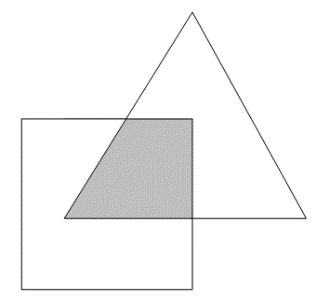
\includegraphics[width=0.3\linewidth]{rwt.png}
    \end{dd}
        \begin{options}
        \item \(2\sqrt[4]{3}\)
        \item \(2\sqrt{3}\) 
        \item \(\sqrt{2\sqrt{3}}\)
        \item 3
    \end{options}
\end{questionbox}

% Masala 15
\begin{questionbox}{15}
    Agar \(3f(x) = f(x+1) + f(x-1)\), \(f(1)=3\), \(f(2)=4\) bo'lsa, \(f(5)\) sonining nechta tub bo'luvchisi bor?
    \begin{options}
        \item 6
        \item 1
        \item 3
        \item 2
    \end{options}
\end{questionbox}

% Masala 16
\begin{questionbox}{16}
    \(\overline{abc} + \overline{cba} = 1453\) tenglamada \(\overline{abc}\) va \(\overline{cba}\) sonlari uch xonali, \(a, b, c\) — raqamlar. \((a+c)\cdot b\) ni toping.
    \begin{options}
        \item 64
        \item 80
        \item 45
        \item 91
    \end{options}
\end{questionbox}

% Masala 17
\begin{questionbox}{17}
    Besh ta bir xil kartochkaga O, B, M, K, R harflari yozilgan (takrorlanishsiz). Kartochkalar aralashtirilib, birma-bir olinadi. Olingan harflar ketma-ketligida «BOR» so'zi hosil bo'lish ehtimolini toping.
    \begin{options}
        \item \(\frac{1}{60}\)
        \item \(\frac{1}{30}\)
        \item \(\frac{1}{40}\)
        \item \(\frac{1}{120}\)
    \end{options}
\end{questionbox}

% Masala 18
\begin{questionbox}{18}
    \(ABC\) uchburchakda (rasm) \(AD \perp BC\), \(AD\) — bissektrisa, \(|BD| = |EC|\), \(\angle EBC = 20^\circ\). \(\angle BCA\) ni toping.
\begin{dd}
        \centering
        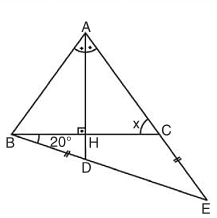
\includegraphics[width=0.3\linewidth]{wfg.png}
    \end{dd}
        \begin{options}
        \item \(45^\circ\)
        \item \(50^\circ\)
        \item \(55^\circ\)
        \item \(60^\circ\)
    \end{options}
\end{questionbox}

% Masala 19
\begin{questionbox}{19}
    Metall sharni bo'yash uchun 100 g bo'yoq sarflandi. Agar shar diametri 4 marta oshirilsa, necha kilogramm bo'yoq kerak bo'ladi?
    \begin{options}
        \item 2,4 kg
        \item 3 kg
        \item 1,6 kg
        \item 1,8 kg
    \end{options}
\end{questionbox}

% Masala 20
\begin{questionbox}{20}
    Yarim aylana va \(ABC\) uchburchak berilgan, \(AB \perp AC\), \(BD = 3\), \(BE = 1\). \(FC : AF\) ni toping.
\begin{dd}
        \centering
        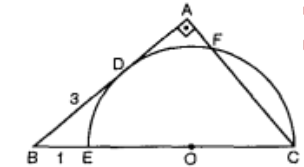
\includegraphics[width=0.5\linewidth]{hdjfj.png}
    \end{dd}
        \begin{options}
        \item 9
        \item 8
        \item 7
        \item 6
    \end{options}
\end{questionbox}

% Masala 21
\begin{questionbox}{21}
    \(y = \ln^2 x - \ln x\) funksiya \(Ox\) o'qini ikki nuqtada kesib o'tadi. Shu nuqtalar va funksiya grafigining minimum nuqtasi hosil qilgan uchburchak yuzini toping.
    \begin{options}
        \item \(\frac{e^2 - 1}{2}\)
        \item \(\frac{e - 1}{4}\)
        \item \(\frac{e - 1}{8}\)
        \item \(\frac{e}{4}\)
    \end{options}
\end{questionbox}

% Masala 22
\begin{questionbox}{22}
    Hisoblang: \(2\arctg\frac{1}{4} + \arctg\frac{7}{23}\).
    \begin{options}
        \item \(\frac{\pi}{4}\)
        \item \(\frac{3\pi}{4}\)
        \item \(\frac{\pi}{3}\)
        \item \(\frac{\pi}{6}\)
    \end{options}
\end{questionbox}

% Masala 23
\begin{questionbox}{23}
    Tenglama yechimlari ko'paytmasini toping:
    \[
    y^2 + 2\sqrt{y^2 + 3y - 4} - 4 + 3y = 0.
    \]
    \begin{options}
        \item 4
        \item \(-1\)
        \item \(-4\)
        \item 1
    \end{options}
\end{questionbox}

% Masala 24
\begin{questionbox}{24}
    \(AB\) — diametr, \(\angle ACE = 30^\circ\), \(\angle EDB = 40^\circ\). \(\angle ABD = \alpha\) ni toping.
\begin{dd}
        \centering
        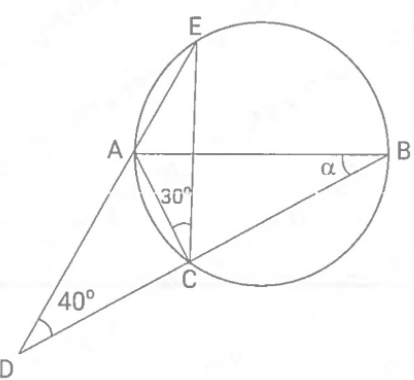
\includegraphics[width=0.3\linewidth]{thjh.png}
    \end{dd}
        \begin{options}
        \item \(15^\circ\)
        \item \(20^\circ\)
        \item \(25^\circ\)
        \item \(30^\circ\)
    \end{options}
\end{questionbox}

% Masala 25
\begin{questionbox}{25}
    5, 7, 11, 17, … sonlari shundayki, qo'shni hadlarining ayirmalari arifmetik progressiya hosil qiladi. Ketma-ketlikning 100-hadini toping.
    \begin{options}
        \item 9605
        \item 9905
        \item 9745
        \item 10095
    \end{options}
\end{questionbox}

% Masala 26
\begin{questionbox}{26}
    Tengsizlikni yeching: \(4x \cdot \arccos(x^2 - 4x + 5) > x^2\).
    \begin{options}
        \item \(\{2\}\)
        \item \((1; 5)\)
        \item \((-2; 3)\)
        \item \(\varnothing\)
    \end{options}
\end{questionbox}

% Masala 27
\begin{questionbox}{27}
    Uchburchak uchun \(\frac{a}{\cos A} = \frac{b}{\cos B}\) tenglik bajariladi. Uchburchak turini aniqlang.
    \begin{options}
        \item muntazam
        \item teng yonli
        \item mavjud emas
        \item o'tmas burchakli
    \end{options}
\end{questionbox}

% Masala 28
\begin{questionbox}{28}
    \(ABCD\) — kvadrat, \(EH \perp DF\), \(AE = EB = EH = 3\). \(BF/FC\) ni toping.
\begin{dd}
        \centering
        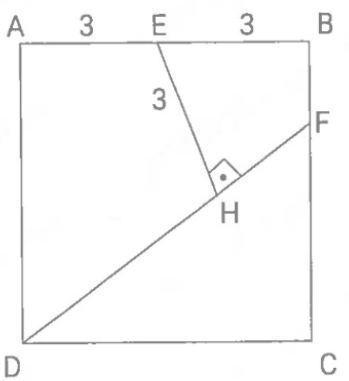
\includegraphics[width=0.3\linewidth]{gaa.png}
    \end{dd}
        \begin{options}
        \item \(\frac{1}{3}\)
        \item \(\frac{1}{2}\)
        \item \(\frac{2}{5}\)
        \item \(\frac{1}{4}\)
    \end{options}
\end{questionbox}

% Masala 29
\begin{questionbox}{29}
    Yig'indini toping:
    \[
    1\cdot 3 + 3\cdot 3^2 + 5\cdot 3^3 + \dots + 93\cdot 3^{47}.
    \]
    \begin{options}
        \item \(47\cdot 3^{47} + 3\)
        \item \(46\cdot 3^{48} + 3\)
        \item \(48\cdot 3^{49} + 3\)
        \item \(46\cdot 3^{46} + 1\)
    \end{options}
\end{questionbox}

% Masala 30
\begin{questionbox}{30}
    \(a_0, a_1, a_2, \dots\) ketma-ketlik uchun \(a_0 = 1\) va \(a_{n+1} = 3a_n-a_{n-1}\) berilgan. \(8a_1 -a_{3}\) ni toping.
    \begin{options}
        \item 12
        \item 13
        \item 3
        \item 2
    \end{options}
\end{questionbox}

% Masala 31
\begin{questionbox}{31}
    Radiusi \(R=1\) bo'lgan aylanaga yuzi 5 ga teng tengyonli trapetsiya tashqi chizilgan. Uchlari aylananing trapetsiyaga urinish nuqtalarida bo'lgan to'rtburchak yuzini toping.
    \begin{options}
        \item 1,6
        \item 1,7
        \item 1,8
        \item 1,9
    \end{options}
\end{questionbox}

% Masala 32
\begin{questionbox}{32}
    \(x^2 - (m+4)x + 2m + 5 = 0\) tenglama uchun \(x_1 < 3 < x_2\) ekanligi ma'lum. \(m\) ning oraliqlarini toping.
    \begin{options}
        \item \((-2; 2)\)
        \item \((2; +\infty)\)
        \item \((-\infty; -2)\)
        \item \((-2; 0)\)
    \end{options}
\end{questionbox}

% Masala 33
\begin{questionbox}{33}
    \(A = \{1,2,3,4,5,6,7\}\), \(B = \{1,2,4,5,7\}\), \(C = \{3,4,6,8\}\) to'plamlar berilgan. \(A \setminus (B \cup C)\) ni toping.
    \begin{options}
        \item \(\{8\}\)
        \item \(\{4\}\)
        \item \(\{4,8\}\)
        \item \(\varnothing\)
    \end{options}
\end{questionbox}

% Masala 34
\begin{questionbox}{34}
    \(ABC\) uchburchakda \(AD\) — bissektrisa, \(AE\) — balandlik. \(\angle ABC - \angle ACB = 28^\circ\) ekanligi ma'lum. \(\angle DAE\) ni toping (gradusda).
    \begin{options}
        \item 13
        \item 14
        \item 15
        \item Aniqlab bo'lmaydi
    \end{options}
\end{questionbox}

% Masala 35
\begin{questionbox}{35}
    \(A(0;12)\), \(C(6;0)\) nuqtalar berilgan. \(S_{OBC}\) ni toping.
\begin{dd}
        \centering
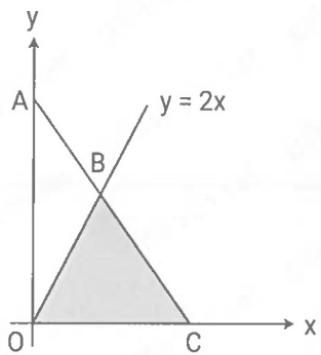
\includegraphics[width=0.3\linewidth]{daf2.png}
    \end{dd}
        \begin{options}
        \item 12
        \item 15
        \item 18
        \item 24
    \end{options}
\end{questionbox}

\end{document}
